\documentclass[border=5pt]{standalone}
\usepackage[utf8]{inputenc}
\usepackage{amsmath}
\usepackage{tikz}
\usetikzlibrary{positioning, fit, shapes}
\usetikzlibrary{chains}
\usetikzlibrary{calc}
\usetikzlibrary{decorations.pathmorphing}
\usetikzlibrary{shapes.multipart}
\usetikzlibrary{decorations,arrows}
\usetikzlibrary{decorations.pathmorphing}
\usepgflibrary{decorations.pathreplacing} 

\begin{document}

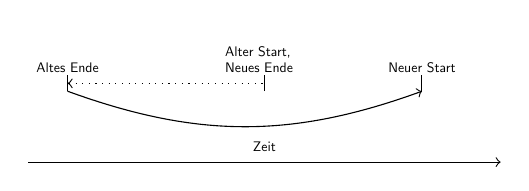
\begin{tikzpicture}[node distance=0cm, font=\sffamily]

% Manually size the picture
\draw[opacity=0] (0, 0) -- (0, 1.7);

% Start bar
\node[scale=0.5, text width=2cm] at (3, 1.3) {Alter Start, \\ Neues Ende};
\draw (3, 0.9) -- (3, 1.1);

% Search orientation
%\node[scale=0.5] at (1.75, 1.2) {Suchrichtung};
\draw[<-, dotted] (0.5, 1) -- (3, 1);

% End bar
\node[scale=0.5] at (0.5, 1.2) {Altes Ende};
\draw (0.5, 0.9) -- (0.5, 1.1);

% New start bar
\node[scale=0.5] at (5, 1.2) {Neuer Start};
\draw (5, 0.9) -- (5, 1.1);

% Arrow to new start
%\draw[<-, dotted] (4, 1) -- (5, 1);
\draw[->] (0.5, 0.9) to [out=-20,in=-160] (5, 0.9);

% Time axis
\node[scale=0.5] at (3, 0.2) {Zeit};
\draw[->] (0, 0) -- (6, 0);

\end{tikzpicture}

\end{document}
